\documentclass[11pt,a4paper,oneside]{report}
\usepackage[a4paper,margin=24mm,headheight=15pt,footskip=12mm]{geometry}
\usepackage[T1]{fontenc}
\usepackage{lmodern}
\usepackage{microtype}
\usepackage{setspace}
\usepackage{graphicx}
\usepackage{booktabs}
\usepackage{longtable}
\usepackage{array}
\usepackage{tabularx}
\usepackage{ragged2e}
\usepackage{enumitem}
\usepackage{xcolor}
\usepackage{listings}
\usepackage{hyperref}
\usepackage{caption}
\usepackage{fancyhdr}
\usepackage{amsmath,amssymb}
\usepackage{url}
\usepackage[none]{hyphenat}

\definecolor{MarketNavy}{HTML}{17324D}
\definecolor{MarketTeal}{HTML}{287D83}
\definecolor{MarketPale}{HTML}{E8F2F3}
\definecolor{MarketGray}{HTML}{F3F6F8}
\hypersetup{colorlinks=true,linkcolor=MarketTeal,urlcolor=MarketTeal,citecolor=MarketTeal,
 pdftitle={MarketNest: Real-World Database System Design and Implementation},
 pdfauthor={Mustakim Al Siyam}}
\setstretch{1.16}
\setlength{\parindent}{0pt}
\setlength{\parskip}{5pt}
\setlength{\emergencystretch}{2em}
\hyphenpenalty=10000
\exhyphenpenalty=10000
\sloppy
\renewcommand{\arraystretch}{1.18}
\setlist[itemize]{leftmargin=1.5em,itemsep=2pt,topsep=3pt}
\setlist[enumerate]{leftmargin=1.7em,itemsep=2pt,topsep=3pt}
\pagestyle{fancy}
\fancyhf{}
\fancyhead[L]{\small MARKETNEST | DATABASE SYSTEM}
\fancyhead[R]{\small ECE 2216}
\fancyfoot[C]{\thepage}
\renewcommand{\headrulewidth}{0.35pt}
\renewcommand{\footrulewidth}{0pt}
\captionsetup{font=small,labelfont=bf,skip=5pt}
\urlstyle{tt}
\def\UrlBreaks{\do\.\do\-\do\_\do\/\do\,}
\newcolumntype{P}[1]{>{\RaggedRight\arraybackslash}p{#1}}
\newcolumntype{Y}{>{\RaggedRight\arraybackslash}X}
\lstdefinestyle{sqlstyle}{language=SQL,basicstyle=\ttfamily\small,
 keywordstyle=\color{MarketTeal}\bfseries,commentstyle=\color{gray},
 stringstyle=\color{red!55!black},numbers=left,numberstyle=\tiny\color{gray},
 breaklines=true,breakatwhitespace=true,frame=single,columns=fullflexible,
 showstringspaces=false,keepspaces=true,tabsize=2,aboveskip=5pt,belowskip=5pt}
\lstset{style=sqlstyle}
\newcommand{\projectpath}[1]{\path{#1}}
\newcommand{\figpage}[2]{%
  \clearpage\thispagestyle{fancy}%
  \begin{center}
  \includegraphics[width=0.96\textwidth,height=0.70\textheight,keepaspectratio]{#1}%
  \end{center}%
  \refstepcounter{figure}%
  \addcontentsline{lof}{figure}{\protect\numberline{\thefigure}#2}%
  \clearpage}
\begin{document}
\begin{titlepage}
\thispagestyle{empty}
\centering
\vspace*{7mm}
{\Large\bfseries Rajshahi University of Engineering \& Technology\par}
\vspace{3mm}
{\large Department of Electrical and Computer Engineering\par}
\vspace{3mm}

\includegraphics[height=42mm,keepaspectratio]{assets/ruet_logo.png}\par
\vspace{14mm}
{\Huge\bfseries\color{MarketNavy} MarketNest\par}
\vspace{5mm}
{\LARGE Real-World Database System Design and Implementation\par}
\vspace{7mm}
{\Large Multi-Vendor E-Commerce Database Management System\par}
\vspace{12mm}
{\large ECE 2216 -- Database Systems Project\par}
\vfill
\begin{tabular}{>{\bfseries}r >{\RaggedRight\arraybackslash}p{0.68\textwidth}}
Submitted by: & Mustakim Al Siyam\\
Student ID: & 2310047\\
Registration No.: & 1100\\
Submitted to: & Md. Rakibul Islam\\
 & Lecturer\\
 & Department of Electronics \& Telecommunication Engineering\\
Submission date: & 10 November 2026\\
\end{tabular}
\vfill
\end{titlepage}

\pagenumbering{roman}
\tableofcontents
\listoffigures
\listoftables
\clearpage
\pagenumbering{arabic}

% The seven main chapters follow the structure in the ECE 2216 project brief.
\chapter{Introduction}
\section{Problem Statement}
Small and medium-sized sellers may manage products, customers, orders, and delivery information through separate spreadsheets, messages, and marketplace tools. This fragmented approach can cause inconsistent stock quantities, outdated prices, duplicated records, unclear payment and delivery status, and difficulty calculating seller commissions and payouts. Customers may consequently receive unreliable information about availability, order progress, and returns.

MarketNest is a multi-vendor e-commerce marketplace in which independent sellers list products and customers purchase products through a common checkout process. The platform records orders, payment attempts, courier shipments, returns, reviews, and seller settlements in a centralized relational database. The database is intended to maintain consistency and support the main operational and reporting activities of the marketplace.

\section{Motivation and System Selection}
A multi-vendor marketplace is sufficiently complex for demonstrating relational database concepts. Its operations involve multiple related entity sets, one-to-many and many-to-many relationships, composite keys, hierarchical categories, historical order-line data, and financial records. In particular, the system must preserve the price paid at checkout even if a seller changes the current catalogue price later.

\section{Objectives}
\begin{enumerate}
 \item Store customer, seller, product, order, payment, shipment, review, return, and payout information in structured relations.
 \item Maintain variant-level prices and stock quantities and prevent negative stock.
 \item Preserve historical purchase prices and the delivery address selected for each order.
 \item Support cart, wishlist, checkout, payment recording, fulfilment, review, and return workflows.
 \item Calculate seller commissions and payouts from delivered sales.
 \item Enforce data integrity using keys, constraints, triggers, procedures, and transactions.
 \item Provide operational searches, reports, and visualizations through a dashboard.
\end{enumerate}

\section{Scope and System Boundary}
The implementation uses synthetic sample data and a locally configured MySQL database. It demonstrates core marketplace database operations. It does not connect to a real payment gateway, execute courier bookings, authenticate dashboard users, calculate live carrier charges, support multi-warehouse inventory, or provide a complete bank settlement and refund ledger. Payment records are stored locally for demonstration; no card details are stored.

\section{System Users}
\begin{longtable}{P{0.25\textwidth}P{0.67\textwidth}}
\toprule
\textbf{User or actor} & \textbf{Main responsibilities}\\\midrule
Customer & Searches products, manages addresses, cart and wishlist, places orders, views delivery progress, reviews delivered items, and requests returns.\\
Seller & Maintains store and product listings, creates variants, updates price and stock, inspects sales, and reviews commission and payout information.\\
Administrator & Oversees seller and catalogue records, categories, coupons, couriers, orders, returns, payouts, and marketplace reports.\\
Courier staff & Updates shipment and delivery status for parcels assigned to the courier company.\\
Payment service (conceptual external actor) & In a real deployment, returns payment-attempt outcomes and transaction references. In this project, outcomes are recorded locally rather than obtained from a live gateway.\\
\bottomrule
\end{longtable}

\section{Functional Requirements}
\begin{enumerate}
 \item Maintain customer and seller records and customer delivery addresses.
 \item Maintain categories, seller-owned products, and product variants with unique SKU, price, and stock.
 \item Search and filter products by keyword, category, seller, price, and rating.
 \item Create and manage customer carts and wishlists.
 \item Create orders from cart items, apply eligible coupons, calculate totals, and reserve stock.
 \item Record payment attempts, payment method, amount, status, and optional transaction reference.
 \item Support order confirmation, cancellation before shipment, and stock restoration on eligible cancellation.
 \item Record courier, shipment, tracking number, and shipment status.
 \item Permit reviews only for delivered order items.
 \item Process return requests subject to the delivery date and purchased quantity.
 \item Calculate seller gross sales, commission, and net payout for a date range.
 \item Generate operational and analytical reports and visualizations.
 \item Support create, search and filter, update, guarded delete, and reporting operations in the dashboard.
\end{enumerate}

\section{Non-Functional Requirements}
\begin{longtable}{P{0.20\textwidth}P{0.72\textwidth}}
\toprule
\textbf{Quality} & \textbf{Requirement}\\\midrule
Integrity & Keys and constraints prevent invalid references, duplicate identifiers, negative stock, invalid quantities, and invalid monetary values.\\
Consistency & Multi-step checkout and cancellation operations use transactions so partial changes are not committed.\\
Security & Credentials are configured locally; the example environment file contains placeholders. Production authentication and full role separation are outside the current dashboard scope.\\
Performance & Indexes support joins and common filters; views simplify recurring reporting queries.\\
Maintainability & SQL schema, seed data, database features, query set, application, and tests are separated into documented files.\\
Recoverability & Database backups should be taken before destructive maintenance or a clean re-seed.\\
\bottomrule
\end{longtable}

\section{Business Rules}
\begin{enumerate}
 \item Each order belongs to one customer and references an address belonging to that same customer.
 \item A customer may maintain multiple addresses; an address is identified by the customer and its address number.
 \item A customer has at most one cart in the implemented design.
 \item A product belongs to one seller and one category; a seller and a category may each be associated with many products.
 \item A product can have multiple variants. Each variant has its own unique SKU, price, and stock quantity.
 \item Cart items and wishlist items are associative relations that prevent duplicate item pairs.
 \item An order contains order lines; the same product variant cannot be repeated as a separate line in the same order.
 \item Each order line stores the unit price paid at checkout, preserving historical price information.
 \item Stock cannot become negative. A new order line is rejected if requested quantity exceeds available stock.
 \item An eligible cancellation before shipment restores reserved stock.
 \item Coupon validity, minimum spend, discount amount, and usage limit are checked when an order is created.
 \item A review requires delivery and is limited to one review per order line; rating is from 1 to 5.
 \item A return must be requested within seven days of delivery. Non-rejected return quantities cannot exceed the quantity purchased.
 \item Seller commission is deducted from gross sales to calculate net payout. Payout date ranges for one seller cannot overlap.
\end{enumerate}

\chapter{Database Implementation}
\section{Design Method and ER Model}
The conceptual ER design contains 18 meaningful entities and associative relations. It records entity attributes, primary keys, relationship names, cardinalities, participation constraints, weak entities, and identifying relationships. Address, product variant, and order item are modeled with identifying keys; cart items and wishlist items resolve many-to-many relationships. The design meets the brief's requirement for a complete ER model with more than ten meaningful entities.

\figpage{../diagrams/marketnest_conceptual_er.png}{MarketNest conceptual ER diagram. The notation key explains entity types, weak entities, identifying relationships, attributes, keys, participation, and cardinalities.}

\figpage{../diagrams/marketnest_relational_eer.png}{MarketNest relational EER diagram produced from the implemented database design.}

The relational EER diagram maps the conceptual model to the implemented MySQL tables. The detailed table definitions in \projectpath{sql/01_schema.sql} are authoritative where a diagram label is shortened for readability.

\section{Relationship and Cardinality Summary}
\begin{longtable}{P{0.36\textwidth}P{0.17\textwidth}P{0.39\textwidth}}
\toprule
\textbf{Relationship} & \textbf{Cardinality} & \textbf{Interpretation}\\\midrule
CUSTOMERS--ADDRESSES & 1:N & A customer may save multiple addresses; each address belongs to one customer.\\
CUSTOMERS--CARTS & 1:0..1 & A customer has at most one cart in the implemented design.\\
CARTS -- PRODUCT VARIANTS & M:N & Resolved by CART ITEMS, which records quantity.\\
CUSTOMERS--PRODUCTS & M:N & Resolved by WISHLIST\_ITEMS.\\
SELLERS--PRODUCTS & 1:N & Each product is owned by one seller.\\
CATEGORIES--PRODUCTS & 1:N & Each product references one category; a category may contain many products.\\
CATEGORIES--CATEGORIES & 1:N recursive & A category may have child categories.\\
PRODUCTS -- PRODUCT VARIANTS & 1:N & Each variant belongs to one product; a product may have multiple variants.\\
CUSTOMERS--ORDERS & 1:N & Each order belongs to one customer.\\
ORDERS -- ORDER ITEMS & 1:N & Each order line belongs to one order.\\
ORDERS--PAYMENTS & 1:N & An order may have multiple payment attempts.\\
ORDERS--SHIPMENTS & 1:N & An order may be fulfilled in one or more parcels.\\
COURIERS--SHIPMENTS & 1:N & Each shipment is assigned to one courier.\\
ORDER\_ITEMS--REVIEWS & 1:0..1 & A delivered order line may have at most one review.\\
ORDER ITEMS -- RETURN REQUESTS & 1:N & One purchased line may have return requests subject to cumulative quantity rules.\\
SELLERS -- SELLER PAYOUTS & 1:N & A seller may have multiple payout records for non-overlapping periods.\\
\bottomrule
\end{longtable}
\clearpage
\phantomsection
\addcontentsline{toc}{section}{Implemented Relational Schema}
\small
\textbf{Implemented relational schema.} The table lists every attribute, including generated fields, and identifies primary keys, foreign keys, alternate keys, and principal constraints. Detailed data types, defaults, indexes, and named constraints are in the schema SQL file.
\setlength{\tabcolsep}{2pt}
\begin{longtable}{@{}P{39mm}P{117mm}@{}}
\caption{Implemented relational schema, keys, and principal constraints}\label{tab:schema}\\
\toprule
\textbf{Table relation} & \textbf{Attributes, keys and constraints}\\\midrule
\endfirsthead
\toprule
\textbf{Table relation} & \textbf{Attributes, keys and constraints}\\\midrule
\endhead
\bottomrule
\endfoot
\textbf{CUSTOMERS} & \textbf{Attributes:} \texttt{customer\_id}, \texttt{full\_name}, \texttt{email}, \texttt{phone}, \texttt{password\_hash}, \texttt{registered\_on}, \texttt{status}\par\textbf{Primary key:} \texttt{customer\_id}\par\textbf{Foreign / alternate keys:} Alternate key: \texttt{email}\par\textbf{Constraints:} Required name, email, and password hash; status has defined values. \\
\textbf{ADDRESSES} & \textbf{Attributes:} \texttt{customer\_id}, \texttt{address\_no}, \texttt{label}, \texttt{street\_line}, \texttt{city}, \texttt{postal\_code}, \texttt{country}, \texttt{is\_default}, \texttt{default\_customer\_id}\par\textbf{Primary key:} \texttt{customer\_id}, \texttt{address\_no}\par\textbf{Foreign / alternate keys:} \texttt{customer\_id} references CUSTOMERS\par\textbf{Constraints:} Generated default-address key is unique; default flag is 0 or 1. \\
\textbf{SELLERS} & \textbf{Attributes:} \texttt{seller\_id}, \texttt{store\_name}, \texttt{email}, \texttt{phone}, \texttt{tax\_id}, \texttt{commission\_rate}, \texttt{joined\_on}, \texttt{status}\par\textbf{Primary key:} \texttt{seller\_id}\par\textbf{Foreign / alternate keys:} Alternate keys: \texttt{email}, \texttt{tax\_id}\par\textbf{Constraints:} Commission rate is between 0 and 100; status has defined values. \\
\textbf{CATEGORIES} & \textbf{Attributes:} \texttt{category\_id}, \texttt{category\_name}, \texttt{parent\_category\_id}\par\textbf{Primary key:} \texttt{category\_id}\par\textbf{Foreign / alternate keys:} \texttt{parent\_category\_id} references CATEGORIES; alternate key: \texttt{category\_name}\par\textbf{Constraints:} Self-parenting is rejected by triggers. \\
\textbf{PRODUCTS} & \textbf{Attributes:} \texttt{product\_id}, \texttt{seller\_id}, \texttt{category\_id}, \texttt{product\_name}, \texttt{description}, \texttt{brand\_name}, \texttt{status}, \texttt{created\_at}\par\textbf{Primary key:} \texttt{product\_id}\par\textbf{Foreign / alternate keys:} \texttt{seller\_id} references SELLERS; \texttt{category\_id} references CATEGORIES\par\textbf{Constraints:} Seller and category are required; product name/category indexes support search. \\
\textbf{PRODUCT VARIANTS} & \textbf{Attributes:} \texttt{product\_id}, \texttt{variant\_no}, \texttt{sku}, \texttt{color}, \texttt{size}, \texttt{price}, \texttt{stock\_qty}\par\textbf{Primary key:} \texttt{product\_id}, \texttt{variant\_no}\par\textbf{Foreign / alternate keys:} \texttt{product\_id} references PRODUCTS; alternate key: \texttt{sku}\par\textbf{Constraints:} Price and stock are non-negative; SKU is unique. \\
\textbf{CARTS} & \textbf{Attributes:} \texttt{cart\_id}, \texttt{customer\_id}, \texttt{updated\_at}\par\textbf{Primary key:} \texttt{cart\_id}\par\textbf{Foreign / alternate keys:} \texttt{customer\_id} references CUSTOMERS; \texttt{customer\_id} is unique\par\textbf{Constraints:} Enforces at most one cart per customer. \\
\textbf{CART ITEMS} & \textbf{Attributes:} \texttt{cart\_id}, \texttt{product\_id}, \texttt{variant\_no}, \texttt{quantity}, \texttt{added\_at}\par\textbf{Primary key:} \texttt{cart\_id}, \texttt{product\_id}, \texttt{variant\_no}\par\textbf{Foreign / alternate keys:} \texttt{cart\_id} references CARTS; variant key references \texttt{PRODUCT\_VARIANTS}\par\textbf{Constraints:} Quantity must be positive; duplicate cart/variant pairs are prevented by the key. \\
\textbf{WISHLIST ITEMS} & \textbf{Attributes:} \texttt{customer\_id}, \texttt{product\_id}, \texttt{added\_at}\par\textbf{Primary key:} \texttt{customer\_id}, \texttt{product\_id}\par\textbf{Foreign / alternate keys:} \texttt{customer\_id} references CUSTOMERS; \texttt{product\_id} references PRODUCTS\par\textbf{Constraints:} Composite key prevents duplicate saved products. \\
\textbf{COUPONS} & \textbf{Attributes:} \texttt{coupon\_id}, \texttt{code}, \texttt{discount\_type}, \texttt{discount\_value}, \texttt{min\_order\_amount}, \texttt{valid\_from}, \texttt{valid\_to}, \texttt{usage\_limit}\par\textbf{Primary key:} \texttt{coupon\_id}\par\textbf{Foreign / alternate keys:} Alternate key: \texttt{code}\par\textbf{Constraints:} Positive discount and usage limit; percent is at most 100; valid date range and minimum are checked. \\
\textbf{ORDERS} & \textbf{Attributes:} \texttt{order\_id}, \texttt{customer\_id}, \texttt{address\_no}, \texttt{coupon\_id}, \texttt{order\_date}, \texttt{order\_status}, \texttt{subtotal}, \texttt{discount\_amount}, \texttt{shipping\_fee}, \texttt{total\_amount}\par\textbf{Primary key:} \texttt{order\_id}\par\textbf{Foreign / alternate keys:} \texttt{customer\_id} references CUSTOMERS; (\texttt{customer\_id}, \texttt{address\_no}) references ADDRESSES; optional \texttt{coupon\_id} references COUPONS\par\textbf{Constraints:} Amounts are non-negative; discount cannot exceed subtotal; total equals subtotal minus discount plus shipping. \\
\textbf{ORDER ITEMS} & \textbf{Attributes:} \texttt{order\_id}, \texttt{line\_no}, \texttt{product\_id}, \texttt{variant\_no}, \texttt{quantity}, \texttt{unit\_price\_paid}\par\textbf{Primary key:} \texttt{order\_id}, \texttt{line\_no}\par\textbf{Foreign / alternate keys:} \texttt{order\_id} references ORDERS; variant key references PRODUCT\_VARIANTS; alternate key: (\texttt{order\_id}, \texttt{product\_id}, \texttt{variant\_no})\par\textbf{Constraints:} Quantity is positive; paid price is non-negative; variant may occur once per order. \\
\textbf{PAYMENTS} & \textbf{Attributes:} \texttt{payment\_id}, \texttt{order\_id}, \texttt{method}, \texttt{amount}, \texttt{pay\_status}, \texttt{transaction\_ref}, \texttt{paid\_at}\par\textbf{Primary key:} \texttt{payment\_id}\par\textbf{Foreign / alternate keys:} \texttt{order\_id} references ORDERS; alternate key: non-null \texttt{transaction\_ref}\par\textbf{Constraints:} Amount must be positive; payment method and status use defined values. \\
\textbf{COURIERS} & \textbf{Attributes:} \texttt{courier\_id}, \texttt{courier\_name}, \texttt{phone}, \texttt{tracking\_url}\par\textbf{Primary key:} \texttt{courier\_id}\par\textbf{Foreign / alternate keys:} Alternate key: \texttt{courier\_name}\par\textbf{Constraints:} Courier name is required and unique. \\
\textbf{SHIPMENTS} & \textbf{Attributes:} \texttt{shipment\_id}, \texttt{order\_id}, \texttt{courier\_id}, \texttt{tracking\_no}, \texttt{ship\_status}, \texttt{shipped\_at}, \texttt{delivered\_at}\par\textbf{Primary key:} \texttt{shipment\_id}\par\textbf{Foreign / alternate keys:} \texttt{order\_id} references ORDERS; \texttt{courier\_id} references COURIERS; alternate key: \texttt{tracking\_no}\par\textbf{Constraints:} Tracking number is unique; delivery cannot precede shipping. \\
\textbf{REVIEWS} & \textbf{Attributes:} \texttt{review\_id}, \texttt{order\_id}, \texttt{line\_no}, \texttt{rating}, \texttt{title}, \texttt{comment}, \texttt{created\_at}\par\textbf{Primary key:} \texttt{review\_id}\par\textbf{Foreign / alternate keys:} (\texttt{order\_id}, \texttt{line\_no}) references ORDER\_ITEMS; this pair is unique\par\textbf{Constraints:} Rating is 1 to 5; trigger requires a delivered item. \\
\textbf{RETURN REQUESTS} & \textbf{Attributes:} \texttt{return\_id}, \texttt{order\_id}, \texttt{line\_no}, \texttt{quantity}, \texttt{reason}, \texttt{return\_status}, \texttt{refund\_amount}, \texttt{requested\_at}\par\textbf{Primary key:} \texttt{return\_id}\par\textbf{Foreign / alternate keys:} (\texttt{order\_id}, \texttt{line\_no}) references \texttt{ORDER\_ITEMS}\par\textbf{Constraints:} Triggers enforce delivery window, cumulative quantity, and valid status transitions. \\
\textbf{SELLER PAYOUTS} & \textbf{Attributes:} \texttt{payout\_id}, \texttt{seller\_id}, \texttt{period\_start}, \texttt{period\_end}, \texttt{gross\_sales}, \texttt{commission\_amount}, \texttt{net\_amount}, \texttt{payout\_status}, \texttt{paid\_at}\par\textbf{Primary key:} \texttt{payout\_id}\par\textbf{Foreign / alternate keys:} \texttt{seller\_id} references SELLERS; alternate key: (\texttt{seller\_id}, \texttt{period\_start}, \texttt{period\_end})\par\textbf{Constraints:} Commission and net totals are checked; payout periods cannot overlap for a seller. \\
\end{longtable}
\normalsize

\section{Integrity Constraints}
The schema uses all constraint classes required by the brief. Primary keys identify every row; foreign keys enforce valid relationships; \texttt{NOT NULL} marks mandatory attributes; \texttt{UNIQUE} protects identifiers such as email, SKU, coupon code, courier name, and tracking number; \texttt{CHECK} restricts quantities, prices, ratings, commission rates, discounts, and totals; and defaults supply appropriate timestamps and statuses. Triggers and stored procedures enforce cross-row rules such as stock reservation and restoration, lifecycle transitions, delivery eligibility, return limits, coupon calculations, and payout-period overlap.

The order total follows $\text{total} = \text{subtotal} - \text{discount} + \text{shipping}$. A composite foreign key ensures that an order cannot use an address belonging to another customer. A generated unique key supports at most one default address per customer. Multi-row and concurrent operations use transactions or locking. Minimum participation rules, such as requiring an order to contain at least one order item, are validated by the checkout workflow.

\section{Functional Dependencies and Normalization}
A combined order-entry relation is selected to demonstrate normalization. It contains order-header data and a repeating group of purchased product variants. The relation is an instructional view of the marketplace data; the physical schema remains the authoritative implementation.

\subsection{Unnormalized Form and Candidate Key}
\begin{lstlisting}[caption={Illustrative unnormalized order form}]
ORDER_FORM_UNF(
  order_id, order_date, customer_id, customer_name, customer_email,
  address_no, ship_city, ship_postal_code, coupon_code,
  { sku, product_id, product_name, color, size, seller_id,
    seller_name, category_id, category_name, quantity, unit_price_paid }
)
\end{lstlisting}
The braces represent a repeating set of order lines. The candidate key after flattening the lines is $(\text{order\_id},\text{sku})$: a variant may appear on many orders, and an order may contain many variants; the implementation also prevents the same variant from being repeated as a separate line in one order.

The functional dependencies used in this example are:
\begin{longtable}{P{0.10\textwidth}P{0.57\textwidth}P{0.25\textwidth}}
\toprule
\textbf{ID} & \textbf{Functional dependency} & \textbf{Reason}\\\midrule
FD1 & $\text{order\_id} \rightarrow \text{order\_date, customer\_id, address\_no, coupon\_code}$ & One order has one header.\\
FD2 & $\text{customer\_id} \rightarrow \text{customer\_name, customer\_email}$ & Customer ID identifies the customer.\\
FD3 & $(\text{customer\_id},\text{address\_no}) \rightarrow \text{ship\_city, ship\_postal\_code}$ & Address number is scoped to a customer.\\
FD4 & $\text{coupon\_code} \rightarrow \text{discount\_type, discount\_value}$ & Coupon code identifies its rule.\\
FD5 & $\text{sku} \rightarrow \text{product\_id, color, size}$ & SKU identifies a sellable variant.\\
FD6 & $\text{product\_id} \rightarrow \text{product\_name, seller\_id, category\_id}$ & Product ID identifies its listing.\\
FD7 & $\text{seller\_id} \rightarrow \text{seller\_name}$ & Seller ID identifies a seller.\\
FD8 & $\text{category\_id} \rightarrow \text{category\_name}$ & Category ID identifies a category.\\
FD9 & $(\text{order\_id},\text{sku}) \rightarrow \text{quantity, unit\_price\_paid}$ & A variant occurs at most once per order.\\
\bottomrule
\end{longtable}
The closure of $(\text{order\_id},\text{sku})$ determines the order header, customer and address facts, coupon facts, variant and product facts, seller and category names, quantity, and paid price. Neither component alone determines all attributes, so the key is minimal under these dependencies.

\subsection{First Normal Form}
The repeating group is removed by storing one product line per row. Every field contains one atomic value.
\begin{lstlisting}[caption={Order form in first normal form}]
ORDER_FORM_1NF(
 order_id, sku, order_date, customer_id, customer_name, customer_email,
 address_no, ship_city, ship_postal_code, coupon_code,
 discount_type, discount_value, product_id, product_name, color, size,
 seller_id, seller_name, category_id, category_name,
 quantity, unit_price_paid
)
-- Candidate key: (order_id, sku)
\end{lstlisting}
Partial dependencies remain: order-header facts depend only on \texttt{order\_id}, while variant and product facts depend on \texttt{sku}.

\subsection{Second Normal Form}
A relation is in 2NF when it is in 1NF and every non-prime attribute depends on the whole candidate key. The partial dependencies are removed by separating order-header, variant, and order-line facts.
\begin{lstlisting}[caption={Decomposition into second normal form}]
ORDER_HEADER(
 order_id PK, order_date, customer_id, customer_name, customer_email,
 address_no, ship_city, ship_postal_code, coupon_code,
 discount_type, discount_value
)
VARIANT_INFO(
 sku PK, product_id, product_name, color, size,
 seller_id, seller_name, category_id, category_name
)
ORDER_LINE(order_id PK/FK, sku PK/FK, quantity, unit_price_paid)
\end{lstlisting}
The non-key attributes in \texttt{ORDER\_LINE} depend on the complete composite key. Transitive dependencies remain in \texttt{ORDER\_HEADER} and \texttt{VARIANT\_INFO}.

\subsection{Third Normal Form}
The remaining transitive dependencies are removed by separating customer, address, coupon, product, seller, and category descriptions.
\begin{lstlisting}[caption={Illustrative third normal form decomposition}]
CUSTOMER(customer_id PK, customer_name, customer_email)
ADDRESS(customer_id PK/FK, address_no PK, ship_city, ship_postal_code)
COUPON(coupon_code PK, discount_type, discount_value)
ORDERS(order_id PK, order_date, customer_id FK, address_no,
       coupon_code FK, FK(customer_id,address_no) REFERENCES ADDRESS)
ORDER_LINE(order_id PK/FK, sku PK/FK, quantity, unit_price_paid)
PRODUCT_VARIANT(sku PK, product_id FK, color, size)
PRODUCT(product_id PK, product_name, seller_id FK, category_id FK)
SELLER(seller_id PK, seller_name)
CATEGORY(category_id PK, category_name)
\end{lstlisting}
This decomposition separates facts about each entity from order-line facts. The implemented physical schema uses \texttt{coupon\_id} rather than coupon code in \texttt{orders}; it uses \texttt{(order\_id,line\_no)} as the order-line primary key and separately enforces uniqueness of the order/variant combination. The normalization example is a design analysis, not a replacement for the physical schema.

\subsection{BCNF Assessment}
A relation is in BCNF if every non-trivial functional dependency $X\rightarrow Y$ has determinant $X$ as a superkey. For the decomposed relations above, the determinants are candidate keys under the stated dependency set: customer ID (and unique email) for CUSTOMER; $(customer\_id,address\_no)$ for ADDRESS; coupon code for COUPON; order ID for ORDERS; $(order\_id,sku)$ for ORDER\_LINE; SKU for PRODUCT\_VARIANT; product ID for PRODUCT; seller ID for SELLER; and category ID for CATEGORY. Thus, the listed decomposed relations satisfy BCNF under these assumptions. This conclusion is limited to the illustrative relation and stated dependencies.

\section{Sample Data Coverage}
The deterministic synthetic dataset contains at least ten rows in every implemented relation, meeting the project brief's data-volume guideline. The counts below come from the included seed data and report summary.
\begin{table}[htbp]\centering
\caption{Sample row counts for the 18 relations}
\begin{tabular}{lr@{\qquad}lr}\toprule
\textbf{Relation} & \textbf{Rows} & \textbf{Relation} & \textbf{Rows}\\\midrule
customers & 10 & addresses & 15\\
sellers & 10 & categories & 12\\
products & 20 & product\_variants & 30\\
carts & 10 & cart\_items & 20\\
wishlist\_items & 20 & coupons & 10\\
orders & 15 & order\_items & 20\\
payments & 15 & couriers & 10\\
shipments & 13 & reviews & 10\\
return\_requests & 10 & seller\_payouts & 10\\
\bottomrule\end{tabular}
\end{table}
All sample accounts and payment references are synthetic. Customer and seller email addresses use the reserved \texttt{example.test} domain; no card details are included.

\section{Database Setup and File Organization}
The project uses MySQL 8.0.16 or later with InnoDB. MySQL Workbench can be used to run and inspect the scripts. Execute the SQL files in the following order from the project root:
\begin{enumerate}
 \item \projectpath{sql/01_schema.sql} creates/selects the database and the 18 tables.
 \item \projectpath{sql/02_seed_data.sql} inserts deterministic sample records. It is intended for a fresh database because it uses fixed IDs.
 \item \projectpath{sql/03_database_features.sql} installs views, stored procedures, and triggers.
 \item Review or execute \projectpath{sql/04_queries.sql}. \projectpath{sql/05_security_template.sql} is an optional least-privilege template and should be adapted by an administrator.
\end{enumerate}
The feature script can be re-applied to replace its database objects. Back up data before a clean reset or destructive maintenance. Connection credentials are stored in a local \texttt{.env}; the project archive contains only \texttt{.env.example} with placeholders.

\chapter{SQL Queries}
\section{Query Coverage}
The project contains 29 business-focused SQL queries in \projectpath{sql/04_queries.sql}. Each query addresses a marketplace question. The table assigns each query one primary category so the counts sum to 29; three of the five aggregate queries also use \texttt{GROUP BY} with \texttt{HAVING}, satisfying that separate requirement.

\begin{table}[htbp]\centering
\caption{Primary classification of the 29 SQL queries}
\begin{tabularx}{\textwidth}{P{0.26\textwidth}P{0.11\textwidth}P{0.20\textwidth}Y}
\toprule
\textbf{Category} & \textbf{Count} & \textbf{Queries} & \textbf{Concepts demonstrated}\\\midrule
Basic queries & 4 & Q01--Q04 & Selection, filtering, sorting, and range conditions.\\
JOIN queries & 7 & Q05--Q11 & INNER JOIN, LEFT JOIN, and multi-table joins across marketplace relations.\\
Aggregate queries & 5 & Q12--Q16 & COUNT, SUM, AVG, MIN/MAX, grouping; three use GROUP BY and HAVING.\\
Subqueries & 4 & Q17--Q20 & Scalar, derived-table, and existence-based nested queries.\\
Arithmetic and logical & 3 & Q21--Q23 & Computed revenue/commission and combined predicates.\\
Complex analytical & 6 & Q24--Q29 & Common table expressions, rankings, LAG, CUME\_DIST, and return rates.\\\midrule
\textbf{Total} & \textbf{29} & Q01--Q29 & Meets the minimum query count and category requirements.\\
\bottomrule
\end{tabularx}
\end{table}

\section{Business Questions Answered}
\small
\begin{longtable}{P{0.11\textwidth}P{0.75\textwidth}}
\caption{Purpose of each labeled SQL query}\label{tab:querylist}\\
\toprule
\textbf{Query} & \textbf{Question answered}\\\midrule
\endfirsthead
\toprule
\textbf{Query} & \textbf{Question answered}\\\midrule
\endhead
\bottomrule
\endfoot
Q01 & Which active catalogue variants have stock available?\\
Q02 & Which orders were placed during a selected date range?\\
Q03 & Which variants fall within a selected price range?\\
Q04 & Which product variants have low stock?\\
Q05 & What are a customer's order history and selected address?\\
Q06 & Which seller and category are associated with each product and its stock?\\
Q07 & What items were purchased and at what historical unit prices?\\
Q08 & What are the shipment tracking details and courier contacts?\\
Q09 & What payment attempts and totals are associated with each order?\\
Q10 & Which purchased items have return requests and what are their states?\\
Q11 & Which products have no reviews?\\
Q12 & What are delivered sales by seller above a specified threshold?\\
Q13 & Which categories contain multiple product listings?\\
Q14 & What are the monthly order counts and average basket values?\\
Q15 & Which product ratings meet a selected average-rating threshold?\\
Q16 & How many return requests exist in each status?\\
Q17 & Which products are priced above the average product price?\\
Q18 & Which customers exceed the average delivered spend?\\
Q19 & Which sellers have low-stock product variants?\\
Q20 & Which products have delivered sales?\\
Q21 & What are line revenues and the corresponding commission amounts?\\
Q22 & Which orders have pending or failed payment attempts?\\
Q23 & Which active listings have low stock?\\
Q24 & Which products rank highest by delivered quantity?\\
Q25 & How do sellers rank by monthly revenue?\\
Q26 & How does monthly revenue change from the preceding month using LAG?\\
Q27 & How do coupon usage and order values compare?\\
Q28 & How does a customer's spend percentile rank using CUME\_DIST?\\
Q29 & What is the product return rate relative to delivered sales?\\
\end{longtable}
\normalsize
The executable SQL statements are maintained in the project bundle instead of being duplicated in full here. This keeps the report readable and leaves the SQL file as the authoritative runnable implementation.

\chapter{Advanced Database Features}
\section{Views}
Three views provide reusable reporting datasets for the application and SQL analysis.
\begin{longtable}{P{0.35\textwidth}P{0.55\textwidth}}
\toprule
\textbf{View} & \textbf{Purpose}\\\midrule
\projectpath{v_product_catalog} & Combines product, seller, category, variant, stock, and review summary for catalogue searching.\\
\projectpath{v_order_summary} & Presents order totals together with successful payment sums and shipment counts.\\
\projectpath{v_seller_monthly_sales} & Summarizes delivered sales, estimated commission, and net sales by seller and month.\\
\bottomrule
\end{longtable}

\section{Stored Procedures}
Three stored procedures perform multi-step database operations.
\begin{longtable}{P{0.37\textwidth}P{0.53\textwidth}}
\toprule
\textbf{Procedure} & \textbf{Operation}\\\midrule
\projectpath{sp_reserve_order_line} & Locks a variant, checks stock, inserts an order line with its paid price, and decreases stock within the caller's transaction.\\
\projectpath{sp_cancel_order} & Performs an eligible cancellation for an unshipped order and coordinates payment-state changes with stock restoration.\\
\projectpath{sp_generate_seller_payout} & Calculates delivered sales for a seller and inclusive date range, derives commission, inserts a payout, and returns its identifier.\\
\bottomrule
\end{longtable}

\section{Triggers}
Thirteen triggers enforce cross-row rules and state transitions. Their names and roles are summarized below; the full definitions are in \projectpath{sql/03_database_features.sql}.
\small
\begin{longtable}{P{0.37\textwidth}P{0.55\textwidth}}
\toprule
\textbf{Trigger} & \textbf{Responsibility}\\\midrule
\projectpath{bi_orders_validate_coupon} & Checks coupon validity, minimum spend, and discount amount on new orders.\\
\projectpath{bi_order_item_check_stock} & Locks and checks a variant before a new order line is inserted.\\
\projectpath{bu_orders_validate_transition} & Rejects invalid order lifecycle changes and cancellation after shipment.\\
\projectpath{au_orders_restore_cancelled_stock} & Restores each line's reserved stock after eligible cancellation.\\
\projectpath{bi_reviews_require_delivery} & Requires the related order item to have been delivered before review.\\
\projectpath{bi_returns_validate_request} & Checks delivery, the seven-day request window, and cumulative return quantity.\\
\projectpath{bu_returns_validate_quantity} & Preserves the purchased-quantity limit when a return request is updated.\\
\projectpath{bu_returns_validate_transition} & Restricts return status changes to the allowed lifecycle.\\
\projectpath{au_returns_restock_refunded} & Restores returned inventory when an approved return is refunded.\\
\projectpath{bi_payouts_no_overlap} & Rejects overlapping payout periods when a payout is inserted.\\
\projectpath{bu_payouts_no_overlap} & Rejects overlapping payout periods when a payout is updated.\\
\projectpath{ai_categories_no_self_parent} & Prevents a new category from being its own parent.\\
\projectpath{bu_categories_no_self_parent} & Prevents an update from making a category its own parent.\\
\bottomrule
\end{longtable}
\normalsize

\section{Transaction Processing and Error Handling}
Checkout uses an application-managed transaction. The application records the order and its lines, reserves stock through the stored procedure, records the payment outcome, and clears the cart before commit. If a line has insufficient stock or another required step fails, the application rolls back the whole checkout so partial changes are not retained. Cancellation uses row locking and transaction handling so the order-state change, payment-state change, and stock restoration occur together. Product creation and its first variant are also committed together.

The database returns constraint or trigger errors for invalid input, duplicate values, missing references, and invalid state changes. The application reports the error to the operator and rolls back an active transaction. The interface validates required fields and numeric ranges before submitting changes; foreign keys and database constraints remain the final integrity boundary. Credentials are stored outside the source in a local environment file.

\chapter{Reports and Application}
\section{Application Architecture}
The administrator operations dashboard is implemented in Python with Streamlit and connects to MySQL through the project database module. Connection settings are loaded from a local \texttt{.env} file. The submitted \texttt{.env.example} contains placeholders only. The real local \texttt{.env} file is excluded from the submission archive.

\section{Implemented Operations}
The dashboard demonstrates create, search and filter, update, guarded delete, checkout, inventory, fulfilment, returns, payments, and reporting operations. It supports seller and product creation, category and SKU management, color and size variants, customer and cart maintenance, coupon selection with a live discount and total preview, manual inventory adjustments, order status updates, return/refund handling, reviews, seller payouts, and chart-based reports. A manual Refresh data control reloads saved changes. Records linked to order history are retained when deletion would break historical references.

\section{Reports and Data Visualizations}
The overview presents catalogue and order counts, delivered revenue, low-stock items, monthly revenue, order-status distribution, and recent activity. Additional report views summarize seller sales, pending returns, payment results, inventory, and customer and order activity. The charts and KPI cards use the included synthetic records.

\section{Dashboard Screenshots}
The two screenshots below document representative application workflows. The overview demonstrates the operational dashboard; the checkout view shows the applied coupon, discount, shipping, and updated total before an order is placed.

\begin{figure}[htbp]\centering
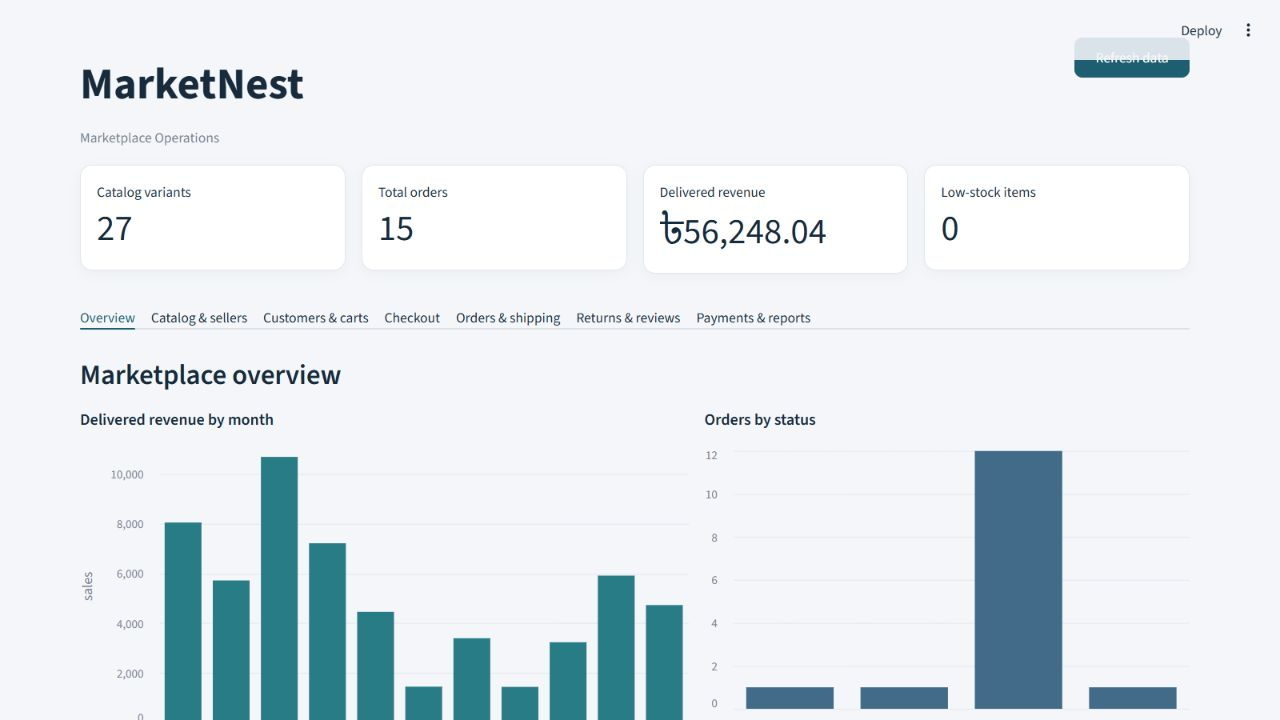
\includegraphics[width=0.94\textwidth,height=0.38\textheight,keepaspectratio]{screenshots/overview.png}
\caption{MarketNest overview with KPI cards, monthly sales, and order-status charts.}
\end{figure}
\begin{figure}[htbp]\centering
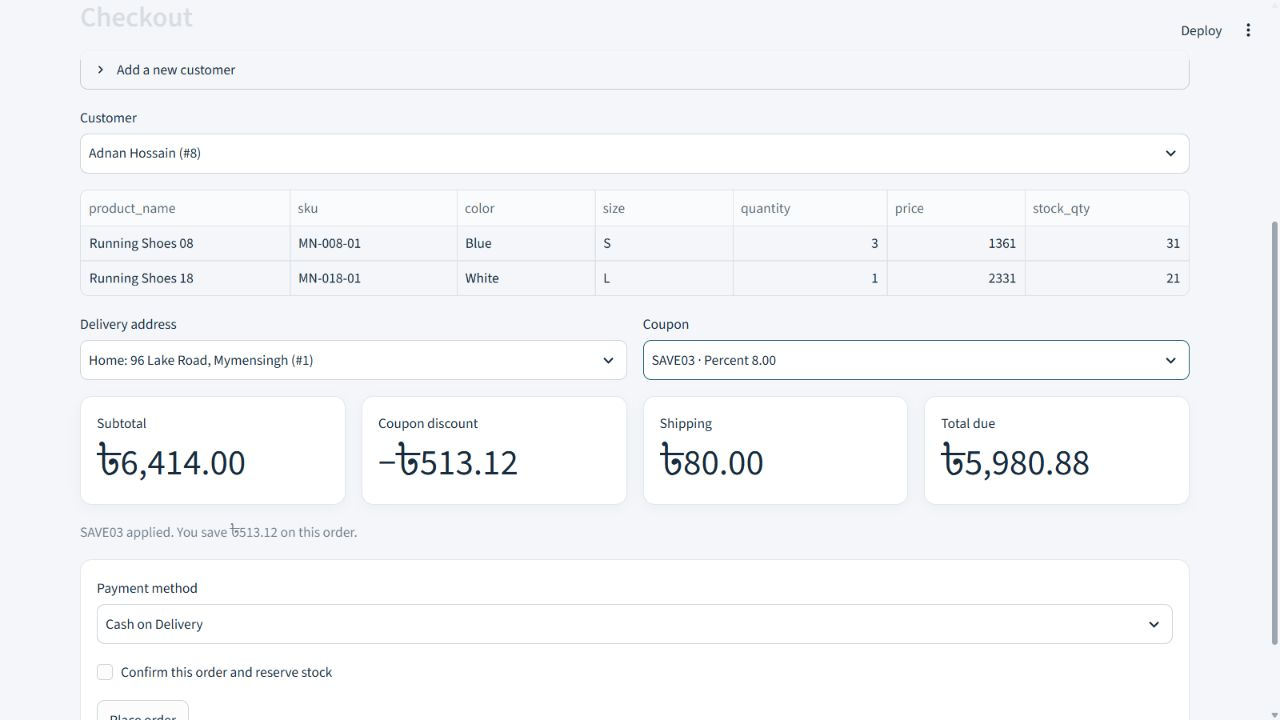
\includegraphics[width=0.94\textwidth,height=0.38\textheight,keepaspectratio]{screenshots/checkout_coupon_preview.png}
\caption{Checkout preview showing coupon savings and the updated total before order placement.}
\end{figure}

\section{System Demonstration}
For a classroom demonstration, the prepared synthetic database can be shown in this sequence:
\begin{enumerate}
 \item Open the overview and explain the KPI cards, sales chart, and order-status summary.
 \item Open the catalogue and create or update a seller, product, and size/color variant.
 \item Search and filter catalogue records, update inventory, and demonstrate guarded deletion.
 \item Select a customer and product variants at checkout; apply a coupon and explain the live subtotal, discount, shipping, and total.
 \item Place an order and show its pending state, then advance it through confirmation and shipment.
 \item Open returns and reviews to show the delivery-window rules and refund workflow.
 \item Open payment and payout reports and explain the seller commission calculation.
 \item Finish by showing the SQL views, constraints, and test results in the project files.
\end{enumerate}
The application runs locally after the SQL scripts are installed, dependencies are installed, and a local \texttt{.env} is configured. The project root README contains the exact launch command and setup steps. The application is an academic operations demonstration; it is not a production marketplace, has no production authentication, and does not connect to a live payment gateway or courier API.

\chapter{Testing}
\section{Test Strategy and Results}
The project documents 34 test cases and includes a Python runner that executes them against a live MySQL instance. Coverage includes valid input, invalid input, duplicate data, foreign-key violations, boundary values, transaction rollback, unauthorized access, triggers, stored procedures, views, and query output. The included observed-results file records 34 PASS and 0 FAIL for the configured MarketNest database on 10 November 2026. The test runner can be run again on another installation; results depend on the installed schema and local database configuration.

\begin{table}[htbp]\centering
\caption{Observed test execution summary}
\begin{tabular}{lrr}\toprule
\textbf{Result} & \textbf{Count} & \textbf{Status}\\\midrule
Passed & 34 & PASS\\
Failed & 0 & PASS\\
\textbf{Total} & \textbf{34} & \textbf{PASS}\\
\bottomrule\end{tabular}
\end{table}

\section{Detailed Test Cases}
Each test case below includes the input or action, expected outcome, observed result, and status specified by the course brief. The detailed CSV files in \projectpath{tests/} are included in the project archive and can be reviewed independently.
\small
\setlength{\tabcolsep}{2pt}
\begin{longtable}{@{}P{13mm}P{51mm}P{92mm}@{}}
\caption{Test case inputs, expected results, observed results, and status}\label{tab:testcases}\\
\toprule
\textbf{Test ID} & \textbf{Input / action} & \textbf{Expected, observed result and status}\\\midrule
\endfirsthead
\toprule
\textbf{Test ID} & \textbf{Input / action} & \textbf{Expected, observed result and status}\\\midrule
\endhead
\bottomrule
\endfoot
TC01 & Count all base tables and rows in the seeded database. & \textbf{Expected:} 18 tables; minimum count >= 10\par\textbf{Observed:} 18 relations checked; minimum row count is 10\par\textbf{Status:} PASS \\
TC02 & Set stock\_qty to -1 for product 1, variant 1. & \textbf{Expected:} CHECK constraint rejects update\par\textbf{Observed:} Database rejected invalid input (error 3819)\par\textbf{Status:} PASS \\
TC03 & Insert a customer using the existing customer01@example.test email. & \textbf{Expected:} UNIQUE constraint rejects insert\par\textbf{Observed:} Database rejected invalid input (error 1062)\par\textbf{Status:} PASS \\
TC04 & Insert a cart item with nonexistent cart\_id 999999. & \textbf{Expected:} Foreign key rejects insert\par\textbf{Observed:} Database rejected invalid input (error 1452)\par\textbf{Status:} PASS \\
TC05 & Insert a product with nonexistent seller\_id 999999. & \textbf{Expected:} Foreign key rejects insert\par\textbf{Observed:} Database rejected invalid input (error 1452)\par\textbf{Status:} PASS \\
TC06 & Insert an order for customer 1 with missing address\_no 999. & \textbf{Expected:} Composite foreign key rejects insert\par\textbf{Observed:} Database rejected invalid input (error 1452)\par\textbf{Status:} PASS \\
TC07 & Insert a product variant using the existing SKU MN-001-01. & \textbf{Expected:} UNIQUE constraint rejects insert\par\textbf{Observed:} Database rejected invalid input (error 1062)\par\textbf{Status:} PASS \\
TC08 & Insert a Percent coupon with discount\_value 150. & \textbf{Expected:} CHECK constraint rejects insert\par\textbf{Observed:} Database rejected invalid input (error 3819)\par\textbf{Status:} PASS \\
TC09 & Insert an order with subtotal 100, shipping 50, and inconsistent total 120. & \textbf{Expected:} CHECK constraint rejects insert\par\textbf{Observed:} Database rejected invalid input (error 3819)\par\textbf{Status:} PASS \\
TC10 & Insert a review with rating 6 (allowed range is 1 to 5). & \textbf{Expected:} CHECK constraint rejects insert\par\textbf{Observed:} Database rejected invalid input (error 3819)\par\textbf{Status:} PASS \\
TC11 & Insert a review for a non-delivered order item (order 15, line 1). & \textbf{Expected:} Trigger rejects insert\par\textbf{Observed:} Database rejected invalid input (error 1644)\par\textbf{Status:} PASS \\
TC12 & Insert a shipment using the existing tracking number TRK-0001. & \textbf{Expected:} UNIQUE constraint rejects insert\par\textbf{Observed:} Database rejected invalid input (error 1062)\par\textbf{Status:} PASS \\
TC13 & Reserve one in-stock variant, check stock decreased by one, then roll back. & \textbf{Expected:} Procedure inserts line and decreases stock\par\textbf{Observed:} Stock decreased by one for an inserted order line; transaction rolled back\par\textbf{Status:} PASS \\
TC14 & Call the reserve procedure with invalid product/variant and quantity 999999. & \textbf{Expected:} Procedure rejects oversell\par\textbf{Observed:} Database rejected invalid input (error 1644)\par\textbf{Status:} PASS \\
TC15 & Check information\_schema for the three required reporting views. & \textbf{Expected:} All 3 views listed in information\_schema\par\textbf{Observed:} All three reporting views are present\par\textbf{Status:} PASS \\
TC16 & Check information\_schema for three procedures and at least 13 triggers. & \textbf{Expected:} 3 procedures and 13 triggers installed\par\textbf{Observed:} Found 3 required procedures and 13 triggers\par\textbf{Status:} PASS \\
TC17 & Call seller payout for seller 1 and 2025 dates; roll back the test. & \textbf{Expected:} Returns a payout ID; test transaction rolls back\par\textbf{Observed:} Payout procedure created a result inside a rolled-back test transaction\par\textbf{Status:} PASS \\
TC18 & Change stock, cause a CHECK failure, and verify rollback restores stock. & \textbf{Expected:} Stock value equals original after rollback\par\textbf{Observed:} Constraint failure was rolled back; original stock remained unchanged\par\textbf{Status:} PASS \\
TC19 & Insert a payment with the existing transaction reference PAY-MN-0001. & \textbf{Expected:} UNIQUE constraint rejects insert\par\textbf{Observed:} Database rejected invalid input (error 1062)\par\textbf{Status:} PASS \\
TC20 & Connect using a deliberately invalid MySQL username and password. & \textbf{Expected:} MySQL denies the deliberately invalid login\par\textbf{Observed:} Database rejected the deliberately invalid account (error 1045)\par\textbf{Status:} PASS \\
TC21 & Request one more return unit than purchased for order 12, line 1. & \textbf{Expected:} Trigger rejects excess quantity\par\textbf{Observed:} Database rejected invalid input (error 1644)\par\textbf{Status:} PASS \\
TC22 & Request a return eight days after delivery for order 12. & \textbf{Expected:} Trigger rejects an expired request\par\textbf{Observed:} Database rejected invalid input (error 1644)\par\textbf{Status:} PASS \\
TC23 & Insert a cart item with quantity zero. & \textbf{Expected:} CHECK constraint rejects quantity zero\par\textbf{Observed:} Database rejected invalid input (error 3819)\par\textbf{Status:} PASS \\
TC24 & Query the catalogue view for variants with available stock. & \textbf{Expected:} At least one available variant is returned\par\textbf{Observed:} Catalog query returned 33 available variants\par\textbf{Status:} PASS \\
TC25 & Update seller 1 payout dates into an overlapping period. & \textbf{Expected:} Trigger rejects overlap with another seller payout\par\textbf{Observed:} Update trigger rejected overlapping payout dates (error 1644)\par\textbf{Status:} PASS \\
TC26 & Update return request 1 quantity to 4, above its purchased quantity. & \textbf{Expected:} Trigger rejects excessive return units\par\textbf{Observed:} Database rejected invalid input (error 1644)\par\textbf{Status:} PASS \\
TC27 & Insert an order with coupon 1 but an incorrect zero discount. & \textbf{Expected:} Trigger rejects an incorrect coupon discount\par\textbf{Observed:} Database rejected invalid input (error 1644)\par\textbf{Status:} PASS \\
TC28 & Insert a category whose parent\_category\_id is its own ID. & \textbf{Expected:} Trigger rejects a category whose parent is itself\par\textbf{Observed:} Database rejected invalid input (error 1644)\par\textbf{Status:} PASS \\
TC29 & Reserve stock and cancel an unshipped order; verify order, payment, and stock, then clean up. & \textbf{Expected:} Procedure cancels an unshipped order, marks payment failed, and restores inventory\par\textbf{Observed:} Cancellation procedure updated order/payment and restored reserved stock\par\textbf{Status:} PASS \\
TC30 & Change order 1 from Delivered to Pending. & \textbf{Expected:} Trigger blocks a Delivered-to-Pending transition\par\textbf{Observed:} Database rejected invalid input (error 1644)\par\textbf{Status:} PASS \\
TC31 & Insert a seller 1 payout for June 2026 overlapping an existing payout. & \textbf{Expected:} Insert trigger rejects an overlapping payout date range\par\textbf{Observed:} Database rejected invalid input (error 1644)\par\textbf{Status:} PASS \\
TC32 & Update category 1 to use itself as its parent. & \textbf{Expected:} Update trigger rejects self-parenting\par\textbf{Observed:} Database rejected invalid input (error 1644)\par\textbf{Status:} PASS \\
TC33 & Refund approved return 4; verify inventory restoration, then roll back. & \textbf{Expected:} Refund transition trigger restores returned inventory\par\textbf{Observed:} Refund transition restored returned units to inventory; transaction rolled back\par\textbf{Status:} PASS \\
TC34 & Change rejected return 7 to Approved. & \textbf{Expected:} Trigger rejects Rejected-to-Approved transition\par\textbf{Observed:} Database rejected invalid input (error 1644)\par\textbf{Status:} PASS \\
\end{longtable}
\normalsize

\section{Test Coverage and Error Handling}
The tests verify that valid stock reservations decrease inventory, a valid cancellation restores it, and rollback preserves the original data after failure. Negative stock, zero quantity, duplicate identifiers, invalid references, invalid totals, out-of-range ratings, invalid coupon discounts, self-parenting categories, invalid status transitions, excess return quantities, and out-of-window returns are rejected by database constraints or triggers. A deliberately invalid database account is refused by MySQL. The application displays database validation errors to the operator and rolls back incomplete transactional operations.

\chapter{Conclusion}
\section{Achievements}
MarketNest implements a relational database for a multi-vendor e-commerce marketplace using MySQL and a Python/Streamlit operations dashboard. The project defines 18 meaningful relations, includes synthetic sample records, enforces primary and foreign keys and integrity constraints, and provides 29 business queries, three views, three stored procedures, and thirteen triggers. Transaction handling protects checkout and cancellation workflows. The dashboard demonstrates catalogue, customer, cart, order, shipping, return, review, payment, payout, reporting, and chart operations.

The normalization example documents UNF-to-1NF, 2NF, and 3NF decomposition, with a BCNF assessment under stated functional dependencies. The recorded database test run completed with 34 passing cases. Together, the schema, SQL features, test evidence, and application demonstrate database design, implementation, transaction processing, and integration.

\section{Limitations}
\begin{itemize}
 \item No live external payment gateway is integrated; payment outcomes are stored locally.
 \item No live courier booking or carrier-charge calculation is implemented.
 \item Dashboard users are not authenticated through a production login system.
 \item The demonstration uses synthetic data and a locally configured database account.
 \item Multi-warehouse inventory and a complete bank settlement/refund ledger are outside the current scope.
\end{itemize}

\section{Future Improvements}
Possible extensions include role-based application login, seller-specific access controls, a payment gateway sandbox, courier API integration, stock reservation expiry, audit logs, automated backups, multi-warehouse inventory, and a complete accounting and settlement ledger.

\renewcommand{\bibname}{References}
\begin{thebibliography}{9}
\addcontentsline{toc}{chapter}{References}
\bibitem{brief} ECE 2216, \textit{Real-World Database System Design and Implementation}, course project brief, 2026.
\bibitem{assignment} Mustakim Al Siyam, \textit{MarketNest: Design of a Multi-Vendor E-Commerce Database System}, ECE 2215 assignment report, Rajshahi University of Engineering \& Technology, 2026.
\bibitem{elmasri} R. Elmasri and S. B. Navathe, \textit{Fundamentals of Database Systems}, 7th ed., Pearson, 2016.
\bibitem{silberschatz} A. Silberschatz, H. F. Korth, and S. Sudarshan, \textit{Database System Concepts}, 7th ed., McGraw-Hill, 2020.
\bibitem{mysql} Oracle, \textit{MySQL 8.0 Reference Manual}, \url{https://dev.mysql.com/doc/refman/8.0/en/}.
\bibitem{streamlit} Streamlit, \textit{Streamlit Documentation}, \url{https://docs.streamlit.io/}.
\end{thebibliography}

\end{document}
